\documentclass[letterpaper]{article}
\usepackage{amsmath}
\usepackage{tikz}
\usepackage{epigraph}
\usepackage{lipsum}
\usepackage{hyperref}
\usepackage{tocloft}
\usepackage{graphicx}

\usepackage{setspace, amsmath}

\usepackage[centering,includeheadfoot,margin=2cm]{geometry}
\usepackage{xcolor}
\usepackage{calc,blindtext}

\renewcommand\epigraphflush{flushright}
\renewcommand\epigraphsize{\normalsize}
\setlength\epigraphwidth{0.3\textwidth}

\definecolor{titlepagecolor}{cmyk}{1,.60,0,.40}

\DeclareFixedFont{\titlefont}{T1}{ppl}{b}{it}{1.0in}

\makeatletter
\def\printauthor{%
    {\large \@author}}
\makeatother
\author{%
    Nico Taljaard \\
    10153285 \vspace{20pt} \\
    Gerhard Smit \\
    12282945 \vspace{20pt} \\
    Martin Schoeman \\
    10651994 \\
}

% The following code is borrowed from: http://tex.stackexchange.com/a/86310/10898

\newcommand\titlepagedecoration{%
	\begin{tikzpicture}[remember picture,overlay,shorten >= -10pt]
	
		\coordinate (aux1) at ([yshift=-15pt]current page.north east);
		\coordinate (aux2) at ([yshift=-410pt]current page.north east);
		\coordinate (aux3) at ([xshift=-4.5cm]current page.north east);
		\coordinate (aux4) at ([yshift=-150pt]current page.north east);
		
		\begin{scope}[titlepagecolor!40,line width=12pt,rounded corners=12pt]
			\draw
			  (aux1) -- coordinate (a)
			  ++(225:5) --
			  ++(-45:5.1) coordinate (b);
			\draw[shorten <= -10pt]
			  (aux3) --
			  (a) --
			  (aux1);
			\draw[opacity=0.6,titlepagecolor,shorten <= -10pt]
			  (b) --
			  ++(225:2.2) --
			  ++(-45:2.2);
		\end{scope}
			\draw[titlepagecolor,line width=8pt,rounded corners=8pt,shorten <= -10pt]
			  (aux4) --
			  ++(225:0.8) --
			  ++(-45:0.8);
		\begin{scope}[titlepagecolor!70,line width=6pt,rounded corners=8pt]
			\draw[shorten <= -10pt]
			  (aux2) --
			  ++(225:3) coordinate[pos=0.45] (c) --
			  ++(-45:3.1);
			\draw
			  (aux2) --
			  (c) --
			  ++(135:2.5) --
			  ++(45:2.5) --
			  ++(-45:2.5) coordinate[pos=0.3] (d);   
			\draw 
			  (d) -- +(45:1);
		\end{scope}
	\end{tikzpicture}
}

\begin{document}

\begin{titlepage}

\noindent
\titlefont Laminin \par
\epigraph{ XGame - Derivco \\ Vision \& Scope.}%
{\textit{ 23/05/2014 }\\ \textsc{ }}
\null\vfill
\vspace*{4cm}
\noindent
\hfill
\begin{minipage}{0.35\linewidth}
    \begin{flushright}
        \printauthor
    \end{flushright}
\end{minipage}
%
\begin{minipage}{0.02\linewidth}
    \rule{1pt}{125pt}
\end{minipage}
\titlepagedecoration
\end{titlepage}

% % % % % % % % % % % % % % %
% 							%
%	Remainder of document	%
% 							%
% % % % % % % % % % % % % % % 

	\newpage
		{\LARGE \bf Change Log}\\[2em]
		
		\begin{tabbing}
			\hspace*{2.5cm}\=\hspace*{2.5cm}\=\hspace*{8cm}\=\hspace*{3cm} \kill
			17/05/2014	\> Version 1.0	\> Document Created 							\> Nico Taljaard \\
			19/05/2014  \> Version 1.0  \> Added Vision									\> Martin Schoeman \\
			21/05/2014  \> Version 1.0  \> Added High Level Use Case Diagram			\> Martin Schoeman\\
		\end{tabbing}

	\newpage
		\renewcommand\contentsname{TABLE OF CONTENTS}
		\newcommand\contentsnameLC{\colorbox{blue}{\makebox[\textwidth-2\fboxsep][l]{\bfseries\color{white} Table of Contents}}}
		
		\renewcommand{\cftdot}{}
		\hypersetup{linktocpage}
		\tableofcontents
		
		\begin{flushleft}
			\LARGE\href{https://github.com/njTaljaard/Laminin_CorpseSlasher/}{Git repository: Laminin - Corpse Slasher}
		\end{flushleft}
		
		\newpage
		
		\section*{\colorbox{blue}{\makebox[\textwidth-2\fboxsep][l]{\bfseries\color{white} Vision \& Scope }}} \addcontentsline{toc}{section}{Vision \& Scope}
		\vspace{0.2in}
		
		\subsection*{Vision}
		\addcontentsline{toc}{subsection}{Vision}
		\vspace{0.1in}
		
		The vision of this project is to create a game that supports multiple platforms, for example android devices and windows computers. The game should be connected to a server where game data can be saved and retrieved real time. The user should be able to log in using a custom log in or an OAuth log in that uses social media like Facebook and Twitter. There must also be a live leader board and achievements. It must be able to develop the game in three months. The project must be developed using only open source and freeware technologies.

		
		\vspace{0.2in}
		\subsection*{Scope}
		\addcontentsline{toc}{subsection}{Scope}
		\vspace{0.1in}
		
		
		\vspace{0.2in}
		
		\section*{\colorbox{blue}{\makebox[\textwidth-2\fboxsep][l]{\bfseries\color{white} Limitations \& Exclusions}}} \addcontentsline{toc}{section}{Limitations \& Exclusions}
		\vspace{0.2in}
		
		\subsection*{Limitations}
		\addcontentsline{toc}{subsection}{Limitations}
		\vspace{0.1in}
		
		
		\vspace{0.2in}
		\subsection*{Exclusions}
		\addcontentsline{toc}{subsection}{Exclusions}
		\vspace{0.1in}
		
		
		
		\vspace{0.2in}
				
		\newpage		
		\section*{\colorbox{blue}{\makebox[\textwidth-2\fboxsep][l]{\bfseries\color{white} High-level use case}}} \addcontentsline{toc}{section}{High-level use case}
		
		\vspace{0.2in}
		
		\begin{figure}[ht!]
		\centering
		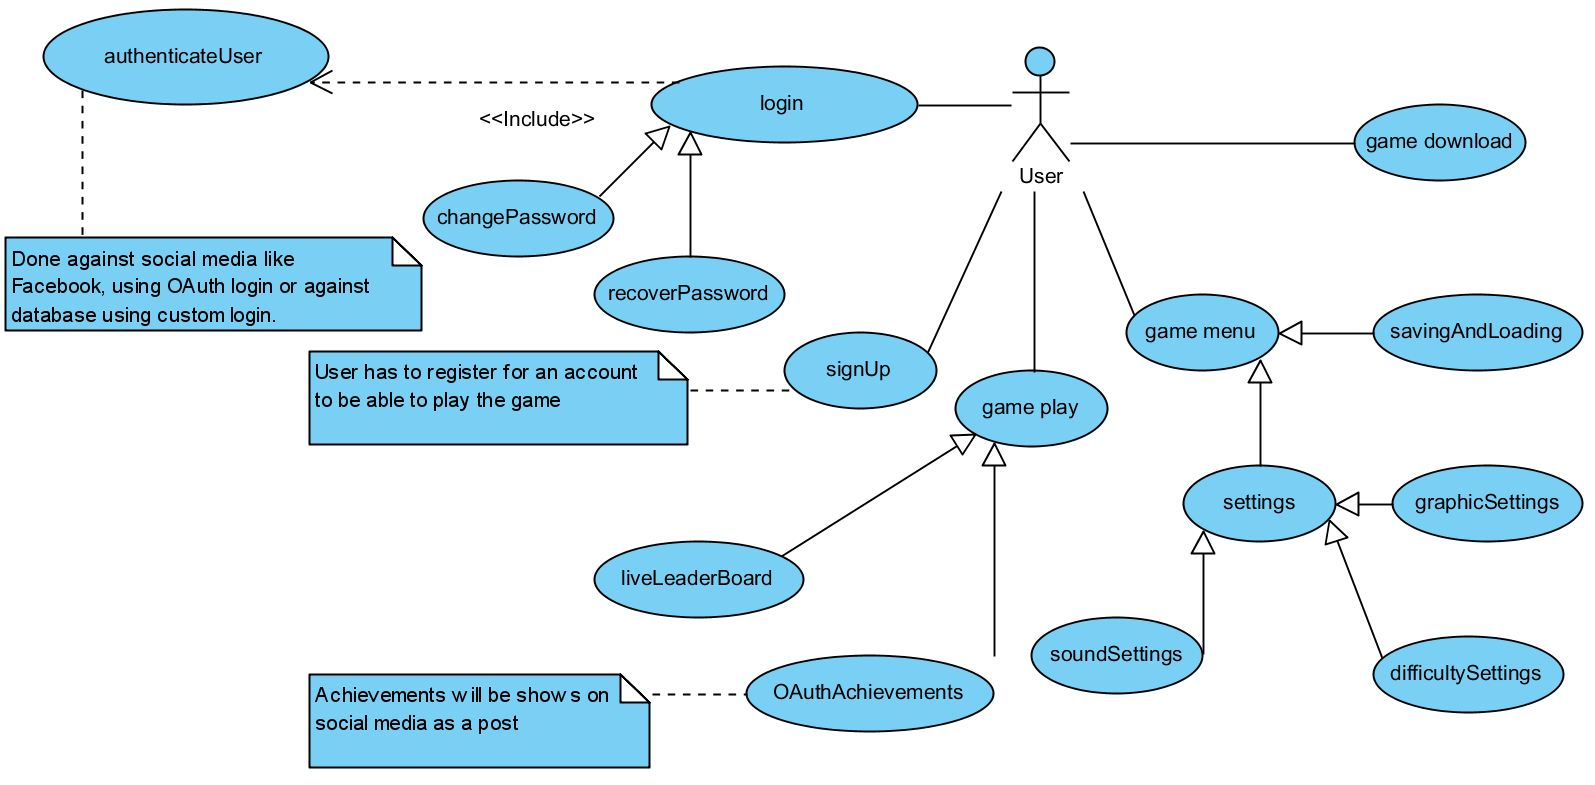
\includegraphics[width=180mm]{high_level_use_case_diagram}
		\caption{High level use case}
		\label{overflow}
		\end{figure}
		
		

\end{document}